%  ProgrammingTips.tex
%  Document created by mw20g10
%  Date created: Sat 05 Apr 2014
%  <+Last Edited: Sat 05 Apr 2014 by mw20g10

\section{Programming Tips}
%Lorem Ipsum\dots
\todo[inline]{Programing Tips section needs completing}

%Outline of what to include (in no particular order):
%\begin{enumerate}
%\item Stack pointer usage
%\item ISR usage - disabled automatically, first instruction should be STF. Final two LDF and RETI.
%\item Sub routine calls and stack frames
%\item General branching (use of CMP)
%\item Any other tips
%\end{enumerate}


This section gives hints and tips about programming for the \samurai{} processor. 

\subsection{Branching}

The \samurai{} processor supports four conditional branches. %Explanation of the branches available.
There are \textbf{BE}, \textbf{BNE}, \textbf{BLT} and \textbf{BGE}.
%These are branch not equal, branch equal, branch greater than or equal and branch less than. 
All conditional branches have an eight bit signed immediate field which is added to the program counter.
Labels are supported by the assembler to aid programming (see section~\ref{sect:assembler}).

All arithmetic operations update the flags based on the result of the operation. 
Logic operations update the negative and zero flags. 
%As well as these, there is a compare and compare immediate (CMP, CMPI) instruction which updates the flag, but the result is not stored. 
As well as these, the \textbf{CMP} and \textbf{CMPI} instructions update the flags, but the result is not stored. 

Conditional branches should be conducted by first doing a logic or arithmetic operation, followed by the relevant branch instruction. 
Listing~\ref{lst:exampleifelse} shows assembly for a simple \textit{if-then-else} clause. 
First, some definitions are made to make the code more readable. 
These are discussed further in section~\ref{sect:assembler}.
A compare is done between the \textit{a} value and an immediate 1. 
If these two numbers are not equal, the program flows takes the jump and loads a 0 into \textit{b}.
Else, the program falls through and a 1 is loaded to the \textit{b} register. 
The program then takes an unconditional jump to the end of the clause. 
This is a simple implementation and can be extended to large case statements.

\lstinputlisting[style=asm,label=lst:exampleifelse,caption={Example code for an \textit{if-then-else} operation.}]{pseudocode/exampleifelse.asm}

Listing~\ref{lst:examplefor} is an example of how to implement a for loop. 
Again, definitions are made give the code more meaning. 
Then the \textit{i} variable is initialised to 0 before the loop. 
Since only greater than or equal, and less than branches are supported, the condition is non-trivial.
This is done by using a temporary register which is set to $i + 1$. 
A compare is done between the temporary register and an immediate 11.
This is as $i \leq 10$ is the same as $(i+1) < 11$. 
A \textbf{BGE} is done to escape the loop. 
If this isn't taken, the contents of the loop is executed.
$i$ is then incremented and the program jumps to the start of the loop. 


%\todo[inline]{If then else example}

\lstinputlisting[style=asm,label=lst:examplefor,caption={Example code for a \textit{for} loop.}]{pseudocode/examplefor.asm}
%\todo[inline]{For and while loop examples}
\todo[inline,color=green]{would a while loop be good to put in?}



\subsection{Stack Pointer Usage}

The \samurai{} processor uses a full descending stack, example usage is held in listing~\ref{lst:exampleSP.asm}.
This means from the initial value the stack pointer is incremented before data is written to memory.
It is recommended that stack pointer is initialised to $x$ where $x-1$ is the top address in main memory. 
A \textbf{PUSH} increments then writes and a \textbf{POP} reads then decrements.
Relative loads from the stack pointer are possible and discussed at length in section~\ref{sec:subroutine_calls}.
\lstinputlisting[style=asm,label=lst:exampleSP,caption={Example code for \textbf{SP} usage.}]{pseudocode/exampleSP.asm}

\subsection{Sub routine calling convention}
\label{sec:subroutine_calls}

Use of a stack frame to pass variables to and from subroutines is recommended when writing assembly for \samurai{}.
This improves code reuse and debugging. 
Example calls for both linked and unlinked subroutines are contained in listing~\ref{lst:exampleSubroutine}
The stack is explained using figure~\ref{fig:stack} which shows the state during the main matter of each subroutine.

Subroutine \emph{one} requires two input parameters and returns a single result.
The caller pushes two register values to the stack and a third dummy value is created by decrementing the stack pointer.
A \textbf{BWL} instruction is used to enter the subroutine.
The callee now has to save the registers it wishes to work with by storing them on the stack.
This subroutine calls another subroutine therefore the first operation should be a \textbf{PUSH LR} which places the link register on the stack.
Five register values are saved then the two input parameters are loaded relative to the stack pointer.
On exit the result is stored at the dummy memory location.
Once all register values are restored it is crucial the link register is also restored before the \textbf{RET} command is used to return the program to the caller. 
The caller does one \textbf{POP} followed by two dummy pops to return the stack its initial state.

Subroutine \emph{two} is called from inside subroutine \emph{one} but because it is a leaf call then the link register does not have to be copied to the stack.
The input parameter is bidirectional and on exit the result is written to the same place from which it was read.

\lstinputlisting[style=asm,label=lst:exampleSubroutine,caption={Example code for calling subroutines.}]{pseudocode/exampleSubroutine.asm}

\begin{figure}[!htb]
	\centering
	\subfigure[Stack state during \emph{one} main matter.]{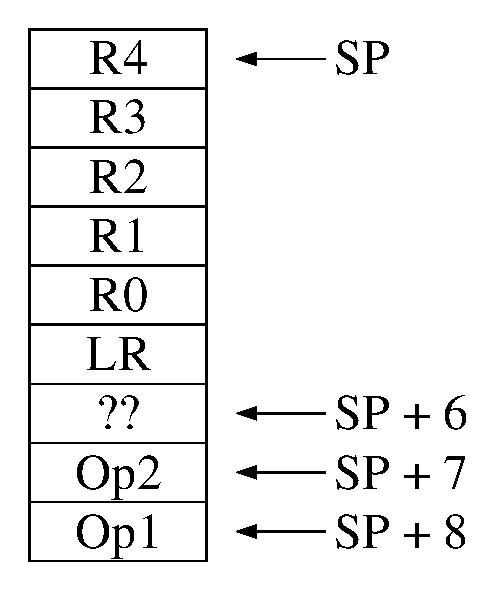
\includegraphics[width=0.3\textwidth]{Figures/oneStack.pdf}
	\label{fig:stack1}}
	\subfigure[Stack state during \emph{two} main matter.]{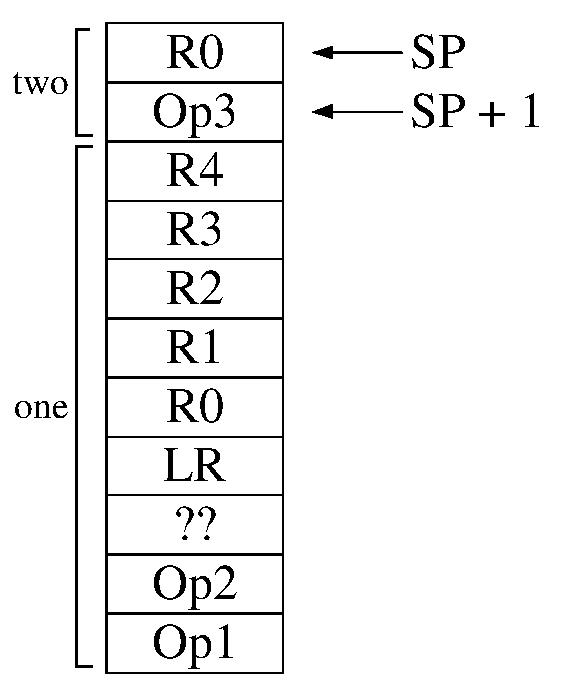
\includegraphics[width=0.3\textwidth]{Figures/twoStack.pdf}
	\label{fig:stack2}}	
	\caption{Stack growth.}
	\label{fig:stack}
\end{figure}




\subsection{Interrupt Service Routines}
%\todo[inline]{Standardise all references to instructions - instructions are now in bold font}

%enabling and disabling interrupts
On reset, interrupts are disabled on the \samurai{} processor.
Two instructions are used to enable and disable interrupts, \textbf{ENAI}, \textbf{DISI}.
These set or clear an internal flag with in the control unit. 
It is not accessible to the user for reading or branching on it's value.
The use of interrupts requires the use of R7 as the stack pointer. 
The stack pointer should be set up before interrupts are enabled in the program.

%When the ISR is triggered
The \textit{nIRQ} signal to the \samurai{} processor is an active low, level triggered signal.
If the interrupt occurs during an instruction, the instruction is completed before the Interrupt Service Routine (ISR) is entered.
The peripheral should hold the \textit{nIRQ} signal low until it has been cleared by the processor.
%The maximum number of clock cycles taken from the nIRQ signal going low until the start of the first instruction in the ISR is started is \todo{insert max time here}.
%This is assuming no latency on a memory access cycles if the previous instruction is a load word. 
\todo[inline,color=green]{Maximum time before ISR is entered.}

Before the ISR is started, the Program Counter value is stored to the stack. 
Also, interrupts are automatically disabled once an interrupt is triggered to prevent the processor being continually interrupted.
Interrupts must be re-enabled before the ISR is completed by the \textbf{ENAI} instruction.
The first instruction in the ISR \textbf{must be} the store flags instruction, \textbf{STF}. 
The final two instructions in the ISR \textbf{must be} load flags \textbf{LDF} and return from interrupt \textbf{RETI}. 
The user is responsible for saving all the registers and restoring them before returning. 

Nested interrupts are supported on the \samurai{} if required. 
The initial interrupt must first be cleared. 
Interrupts can then be re-enabled. 
If a new interrupt occurs, the ISR is run. 
Once the second ISR is completed, the program flow is returned to where it was before hand and the first ISR run is then complete.

The ISR can also conduct a function call. 
However, this is not recommended as the ISR should be short in length.

The general outline for the ISR is:
\begin{enumerate}
\item Store Flags
\item Push registers to stack
\item Clear interrupt source
\item Enable interrupts
\item Process data
\item Restore registers
\item Load Flags
\item Return from Interrupt
\end{enumerate}

%\todo[inline]{repetition here with next section, this is use, the other is warning it's reserved. Therefore OK}
The ISR is implemented by using the ``.isr'' or ``.ISR'' label. 
It can be placed anywhere in the code and be any length.
A general outline in assembly language is shown in listing~\ref{lst:exampleisr}. 
This structure should be followed for the ISR.


\lstinputlisting[style=asm,label=lst:exampleisr,caption={Example outline for the Interrupt Service Routine}]{pseudocode/exampleisr.asm}

\todo[inline,color=green]{If the assembler supports errors about the required instructions, mention this here}
%\todo[inline]{check ISR references. Make the first in full and acronym then on}
\todo[inline]{any more tips sections?}


